%!LW recipe=latexmk-xelatex
\documentclass[compress]{beamer}

\usetheme[block=fill]{metropolis}

\usepackage{graphicx} % Allows including images
\usepackage{amsmath,amsfonts,amsthm,amssymb}
\usepackage{color}
\usepackage{xcolor,cancel}
\usepackage{tcolorbox}
\setbeamercolor{colorBoxStuff}{fg=black, bg=gray!30!white}
%\setitemize{label=\usebeamerfont*{itemize item}%
%	\usebeamercolor[fg]{itemize item}
%	\usebeamertemplate{itemize item}}
\definecolor{mDarkBrown}{HTML}{604c38}
\definecolor{mDarkTeal}{HTML}{23373b}
\definecolor{mLightBrown}{HTML}{EB811B}
\definecolor{mMediumBrown}{HTML}{C87A2F}
\definecolor{mygreen}{HTML}{98C2B9}
\definecolor{myyellow}{HTML}{DFD79C}
\definecolor{myblue}{HTML}{8CA7CC}
\definecolor{kern}{HTML}{8CC2B7}
\newcommand{\blue}[1]{\textcolor{blue}{#1}}


\usepackage{float}
\usepackage{framed}
\usepackage{epsfig}
\usepackage{graphicx}
\usepackage{subcaption}
\usepackage{ulem}
\usepackage{hhline}
\usepackage{multirow}
\usepackage{comment}   
\usepackage{bbm}
\usepackage{tikz}   
\def\Put(#1,#2)#3{\leavevmode\makebox(0,0){\put(#1,#2){#3}}}
\newcommand*\mystrut[1]{\vrule width0pt height0pt depth#1\relax}
\newcommand{\eqdef}{\mathbin{\stackrel{\rm def}{=}}}
\usepackage{hyperref}


\newcommand{\bs}[1]{\boldsymbol{#1}}
\newcommand{\bv}[1]{\mathbf{#1}}
\newcommand{\R}{\mathbb{R}}
\newcommand{\E}{\mathbb{E}}

\DeclareMathOperator*{\argmin}{arg\,min}
\DeclareMathOperator*{\argmax}{arg\,max}
\DeclareMathOperator{\nnz}{nnz}
\DeclareMathOperator{\vol}{vol}
\DeclareMathOperator{\diag}{diag}
\DeclareMathOperator{\Var}{Var}
\DeclareMathOperator{\sinc}{sinc}
\DeclareMathOperator{\sign}{sign}
\DeclareMathOperator{\dist}{dist}
\DeclareMathOperator{\mv}{mv}
\DeclareMathOperator{\sgn}{sgn}
\DeclareMathOperator{\step}{step}
\DeclareMathOperator{\gap}{gap}
\DeclareMathOperator{\poly}{poly}
\DeclareMathOperator{\tr}{tr}
\DeclareMathOperator{\orth}{orth}
\newcommand{\norm}[1]{\|#1\|}
\captionsetup[subfigure]{labelformat=empty}
\captionsetup[figure]{labelformat=empty}
\DeclareMathOperator*{\lmin}{\lambda_{min}}
\DeclareMathOperator*{\lmax}{\lambda_{max}}

\newcommand{\specialcell}[2][c]{%
  \begin{tabular}[#1]{@{}c@{}}#2\end{tabular}}
\newcommand{\specialcellleft}[2][c]{%
\begin{tabular}[#1]{@{}l@{}}#2\end{tabular}
}

\newtheorem{claim}[theorem]{Claim}
%\newtheorem{corollary}[theorem]{Corollary}

\usepackage{tabstackengine}
\stackMath


%----------------------------------------------------------------------------------------
%	TITLE PAGE
%----------------------------------------------------------------------------------------

\title{CS-GY 6763: Lecture 3 \\  Finish Chebyshev's, Exponential Concentration Inequalities}
\author{NYU Tandon School of Engineering, Prof. Christopher Musco}
\date{}

\begin{document}

\begin{frame}
	\titlepage 
\end{frame}

\metroset{titleformat=smallcaps}

\begin{frame}
	\frametitle{distinct elements problem}
\textbf{Input:} $d_1, \ldots, d_n \in \mathcal{U}$ where $\mathcal{U}$ is a huge universe of items. 

	\textbf{Output:} Number of \emph{distinct} inputs, $D$.

\textbf{Example:} $f(1, 10, 2, 4, 9, 2, 10, 4) \rightarrow D = 5$

\vspace{.5em}
\hrule
\vspace{.5em}

\textbf{Flajolet–Martin (simplified)}:
\begin{itemize}
	\item Choose random hash function $h: \mathcal{U} \rightarrow [0,1]$.
	\item $S = 1$ 
	\item For $i = 1, \ldots, n$
	\begin{itemize}
		\item $S \leftarrow \min(S, h(x_i))$
	\end{itemize} 
	\item Return: $\frac{1}{S} - 1$
\end{itemize}
\end{frame}

\begin{frame}
	\frametitle{visualization}
	\small
	\textbf{Flajolet–Martin (simplified)}:
	\vspace{-.5em}
	\begin{itemize}
		\item Choose random hash function $h: \mathcal{U} \rightarrow [0,1]$.
		\vspace{-.25em}
		\item $S = 1$ 
		\vspace{-.25em}
		\item For $i = 1, \ldots, n$
		\vspace{-.25em}
		\begin{itemize}
			\vspace{-.25em}
			\item $S \leftarrow \min(S, h(x_i))$
		\end{itemize} 
		\vspace{-.25em}
		\item Return: $\tilde{D} = \frac{1}{S} - 1$
	\end{itemize}
\vspace{-.5em}
	\begin{center}
	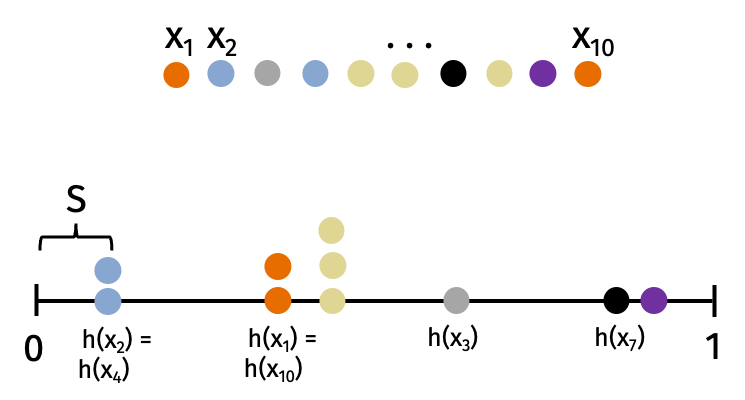
\includegraphics[width=.75\textwidth]{better_minhash_cut.png}
	\end{center}
\end{frame}


\begin{frame}
	\frametitle{proof ``from the book''}
	$\E[S] = \Pr[(D+1)^\text{st} \text{ item has the smallest hash value}]$.
	\begin{center}
			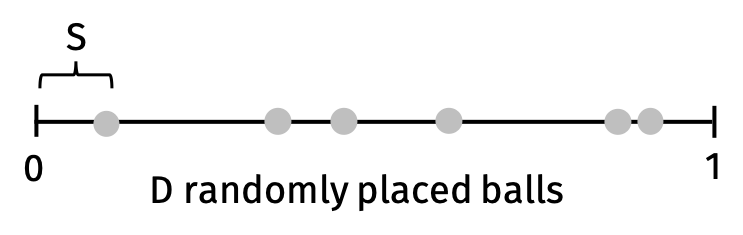
\includegraphics[width=.6\textwidth]{FMimage.png}
	\end{center}
	By symmetry, this equals $\frac{1}{D+1}$ (since every ball is equally likely to be first). 

	\textbf{Final Estimate:} $\tilde{D} = \frac{1}{S} - 1$.
	
\end{frame}


\begin{frame}
	\frametitle{proving concentration}	
	$\E S = \frac{1}{D + 1}$. \textbf{Estimate:} $\tilde{D} = \frac{1}{S} - 1$. \textbf{Claim:} We have for $\epsilon < \frac{1}{2}$:
	
	\begin{center}
	If $(1-\epsilon)\E S \leq S \leq (1+\epsilon)\E S$, then:
	\begin{align*}
	\alert{(1-4\epsilon)D \leq \tilde{D} \leq (1+4\epsilon)D.}
	\end{align*}
	\end{center}
\vspace{10em}

	So, it suffices to show that $S$ concentrates around its mean. I.e. that $|S - \E S| \leq \epsilon\cdot\E S$. We will use Chebyshev's inequality as our concentration bound.
\end{frame}

\begin{frame}
\frametitle{$\epsilon$ manipulation tricks}
\textbf{Recall:}
\begin{align*}
	1+\epsilon \leq \frac{1}{1-\epsilon} \leq 1+ 2\epsilon \text{ for } \epsilon \in [0,.5].
\end{align*}
\begin{align*}
	1-\epsilon \leq \frac{1}{1+\epsilon} \leq 1 - .5\epsilon \text{ for } \epsilon \in [0,1].
\end{align*}
\end{frame}

\begin{frame}
	\frametitle{calculus proof}	
	\begin{lemma}
	$\Var[S] = \E [S^2] - \E[S]^2= \frac{2}{(D+1)(D+2)} - \frac{1}{(D+1)^2} \leq \frac{1}{(D+1)^2}$.
	\end{lemma}
	\textbf{Proof:} 
	\begin{align*}
	\E[S^2] &= \int_0^1 \Pr[S^2 \geq \lambda] d\lambda & &\text{} \\
	&= \int_0^1 \Pr[S \geq \sqrt{\lambda}] d\lambda & &\text{} \\
	&= \int_0^1 (1-\sqrt{\lambda})^D d\lambda & &\text{} \\
	& = \frac{2}{(D+1)(D+2)}& &\text{}
	\end{align*}
	
	\small
	\url{www.wolframalpha.com/input?i=antiderivative+of+\%281-sqrt\%28x\%29\%29\%5ED}
\end{frame}

\begin{frame}
	\frametitle{proof ``from the book''}
	$\E[S^2] = ??$.
	\begin{center}
			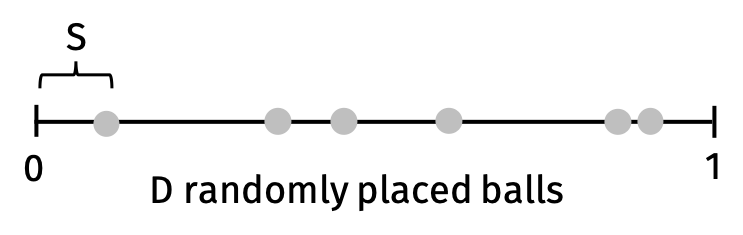
\includegraphics[width=.6\textwidth]{FMimage.png}
	\end{center}
\end{frame}

\begin{frame}
	\frametitle{fm analysis}
	Recall we want to show that, with high probability, $(1-\epsilon) \E[S] \leq S \leq (1-\epsilon) \E[S]$. \vspace{1em}
	\begin{itemize}
		\item $\E[S] = \frac{1}{D+1} = \mu.$ \vspace{.5em}
		\item $\Var[S] \leq \frac{1}{(D+1)^2} = \mu^2$. Standard deviation: $\sigma \leq \mu$. \vspace{.5em}
		\item Want to bound $\Pr[|S - \mu| \geq \epsilon \mu] \leq \delta$. \vspace{.5em}
	\end{itemize}
	
	\textbf{Chebyshev's}: $\Pr[|S - \mu| \geq \epsilon \mu] = \Pr[|S - \mu| \geq \epsilon \sigma] \leq \frac{1}{\epsilon^2}$.
	
	\begin{center}
	\alert{\textbf{Vacuous bound. Our variance is way too high!}}
	\end{center}
\end{frame}


\begin{frame}
	\frametitle{variance reduction}
	\textbf{Trick of the trade:} Repeat many independent trials and take the mean to get a better estimator.
	
	Given i.i.d. (independent, identically distributed) random variables $X_1, \ldots, X_k$ with mean $\mu$ and variance $\sigma^2$, what is:
	\begin{itemize}
		\item $\E\left[\frac{1}{k}\sum_{i=1}^k X_i\right] = $
		\vspace{1em}
		\item $\Var\left[\frac{1}{k}\sum_{i=1}^k X_i\right] = $
	\end{itemize} 
\end{frame}

\begin{frame}
	\frametitle{fm analysis}
	Using independent hash functions, maintain $k$ independent sketches $S_1, \ldots, S_k$.
\vspace{-1em}
\begin{center}
	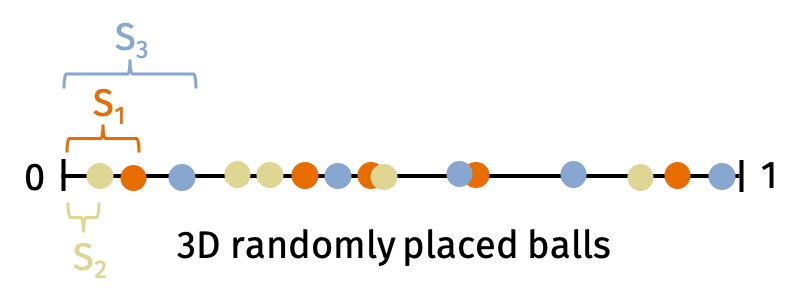
\includegraphics[width=.7\textwidth]{improvedFM.png}
\end{center}

\vspace{-1em}	
\textbf{Flajolet–Martin}:
		\begin{itemize}
			\item Choose $k$ random hash function $h_1, \ldots, h_k: \mathcal{U} \rightarrow [0,1]$.
			\item $S_1 = 1, \ldots, S_k = 1$ 
			\item For $i = 1, \ldots, n$
			\begin{itemize}
				\item $S_j \leftarrow \min(S_j, h_j(x_i))$ for all $j \in 1, \ldots, k$.
			\end{itemize} 
			\item $S = (S_1 + \ldots + S_k)/k$
			\item Return: $\frac{1}{S} - 1$
		\end{itemize}
\end{frame}

\begin{frame}
	\frametitle{fm analysis}
	\textbf{1 estimator}:
	\begin{itemize}
		\item $\E[S] = \frac{1}{D+1} = \mu.$
		\item $\Var[S] = \mu^2$
	\end{itemize}
	\textbf{$k$ estimators}:
	\begin{itemize}
		\item $\E[S] = \frac{1}{D+1} = \mu.$
		\item $\Var[S] \leq  \mu^2/k$
		\item By Chebyshev, $\Pr[|S - \E S| \geq c \mu/\sqrt{k}] \leq \frac{1}{c^2}$.
	\end{itemize}

	Setting $c = 1/\sqrt{\delta}$ and $k = \frac{1}{\epsilon^2\delta}$ gives:
	\begin{align*}
		\Pr[|S - \mu| \geq \epsilon \mu] \leq \delta.
	\end{align*}
\end{frame}

\begin{frame}[t]
	\frametitle{fm analysis}
	\begin{itemize}
		\item Recall that to ensure $(1-\bar{\epsilon}) D \leq \frac{1}{S} - 1 \leq (1+\bar{\epsilon}) D$, we needed  $|S - \mu| \leq \frac{\bar{\epsilon}}{4} \mu$. 
		\item So apply the result from the previous slide with $\epsilon = \bar{\epsilon}/4$. 
		\item Need to store $k = \frac{1}{\epsilon^2\delta} = \frac{1}{(\bar{\epsilon}/4)^2\delta} = \frac{16}{\epsilon^2\delta}$ counters.
	\end{itemize}

	\textbf{Total space complexity}: $\alert{O\left(\frac{1}{\epsilon^2\delta}\right)}$ to estimate distinct elements up to error $\epsilon$ with success probability $1-\delta$.
\end{frame}

\begin{frame}
	\frametitle{note on failure probability}
	$\alert{O\left(\frac{1}{\epsilon^2\delta}\right)}$ space is an impressive bound:
	\begin{itemize}
		\item $1/\epsilon^2$ dependence cannot be improved.
		\item No linear dependence on number of distinct elements $D$.\footnote{Technically, if we account for the bit complexity of storing $S_1, \ldots, S_k$ and the hash functions $h_1, \ldots, h_k$, the space complexity is $O\left(\frac{\log D}{\epsilon^2\delta}\right)$.}
		\item But... $1/\delta$ dependence is not ideal. For $95\%$ success rate, pay a $\frac{1}{5\%} = 20$ factor overhead in space. 
	\end{itemize}
We can get a better bound depending on $O(\log(1/\delta))$ using \emph{exponential tail bounds.} We will see next.
\end{frame}

\begin{frame}
	\frametitle{distinct elements in practice}
	In practice, we cannot hash to real numbers on $[0,1]$. Could use a finite grid, but more popular choice is to hash to integers (bit vectors).
	
	\textbf{Real Flajolet-Martin / HyperLogLog:}
	\begin{columns}
		\begin{column}{.4\textwidth}
			\begin{center}
				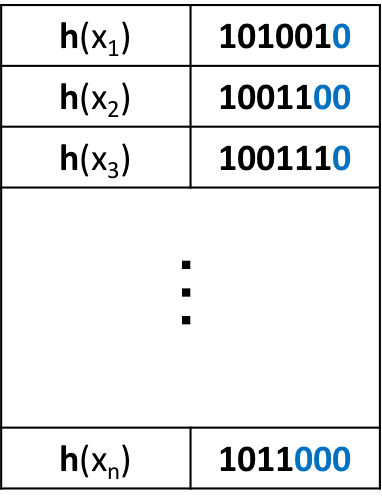
\includegraphics[width=.7\textwidth]{loglog2.png}
			\end{center}
		\end{column}
		\begin{column}{.6\textwidth}
				\begin{itemize}
					\item Estimate \# distinct elements based on maximum number of trailing zeros $\bv m$.
					\item The more distinct hashes we see, the higher we expect this maximum to be.
				\end{itemize}
		\end{column}
	\end{columns}
	\begin{center}
	\end{center}
\end{frame}

\begin{frame}
	\frametitle{loglog space}
	\textbf{Total Space:} $O \left (\frac{\log \log D}{\epsilon^2} + \log D \right )$ for an $\epsilon$ approximate count.
	
	\small ``Using an auxiliary memory smaller than the size of this abstract, the LogLog algorithm makes it possible to estimate in a single pass and within a few percents the number of different words in the whole of Shakespeare’s works.'' -- Flajolet, Durand.
	
	
	\vspace{1em}
	\uncover<3->{
		Using HyperLogLog to count $1$ billion distinct items with $2\%$ accuracy:
		\begin{align*}
			\text{space used } &= O \left (\frac{\log \log D}{\epsilon^2} + \log D \right )\\ \uncover<2->{&= \frac{1.04 \cdot \lceil \log_2 \log_2 D\rceil}{\epsilon^2} + \lceil \log_2 D \rceil \text{ bits}\\}
			\uncover<3->{&= \frac{1.04 \cdot 5}{.02^2} + 30 = 13030\text{ bits} \approx \alert{1.6\ kB}!}
		\end{align*}
	}
\end{frame}

\begin{frame}
	\frametitle{hyperloglog in practice}
	\begin{center} 
		Although, to be fair, storing a dictionary with $1$ billion bits only takes 125 megabytes. Not tiny, but not unreasonable.
		
		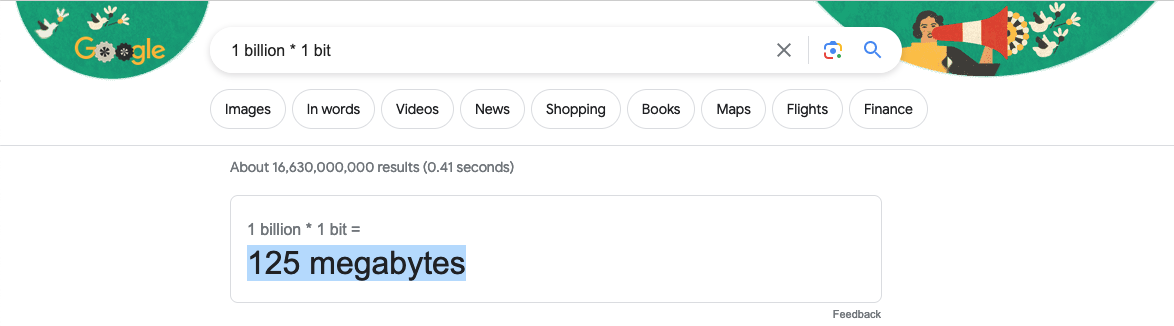
\includegraphics[width=\textwidth]{google_bit_calculations.png}
	\end{center}
	These estimators become more important when you want to count \emph{many} different things (e.g., a software company tracking clicks on 100s of UI elements).
\end{frame}

\begin{frame}
	\frametitle{distributed distinct elements}
	Also very important in distributed settings. 
	\begin{center}
		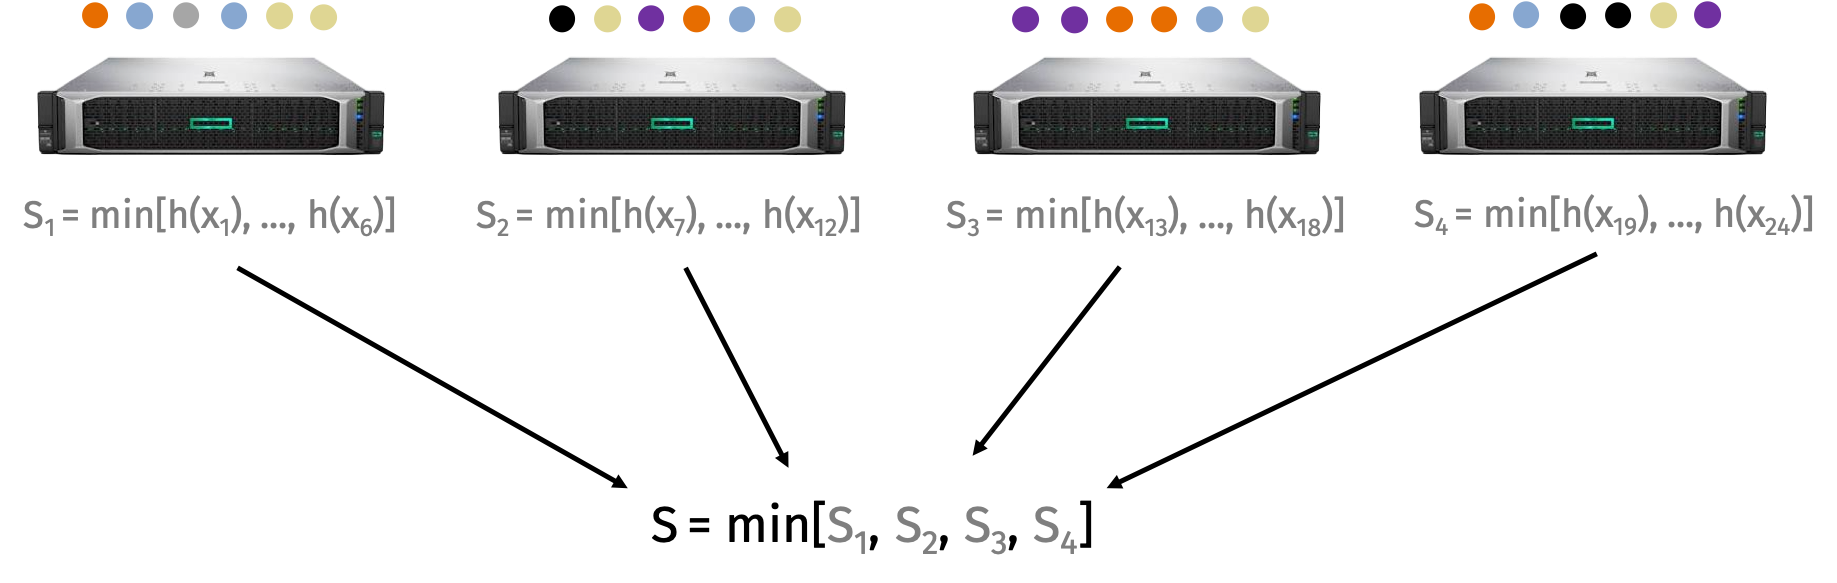
\includegraphics[width=\textwidth]{dist_min_hash.png}
	\end{center}

	Distinct elements summaries are ``mergeable''. No need to share lists of distinct elements if those elements are stored on different machines. Just share minimum hash value.
\end{frame}

\begin{frame}
	\frametitle{hyperloglog in practice}
	\small
	\textbf{Implementations:} Google PowerDrill, Facebook Presto, Twitter Algebird, Amazon Redshift.
	
	\textbf{Use Case:} Exploratory SQL-like queries on tables with $100$'s of billions of rows.
	\begin{itemize}
		\item \alert{Count} number of \alert{distinct} users in Germany that  made at least one search containing the word `auto' in the last month.
		\item \alert{Count} number of \alert{distinct} subject lines in emails sent by users that have registered in the last week.
		% \item \alert{Count} number of \alert{distinct} zip codes in which at least one search has been made for blah
	\end{itemize}
	\uncover<2->{
		\begin{center}
			\textbf{Answering a query requires a (distributed) linear scan over the database: \emph{2 seconds} in Google's distributed implementation.}
			
				\textbf{\alert{Google Paper: ``Processing a Trillion Cells per Mouse Click''}}
		\end{center}
	}
\end{frame}


\begin{frame}
	\frametitle{beyond chebyshev}
	\textbf{Motivating question:} Is Chebyshev's Inequality tight?
	
	It is the worst case, but often not in reality.
	\vspace{-1em}
	\begin{figure}
		\centering
		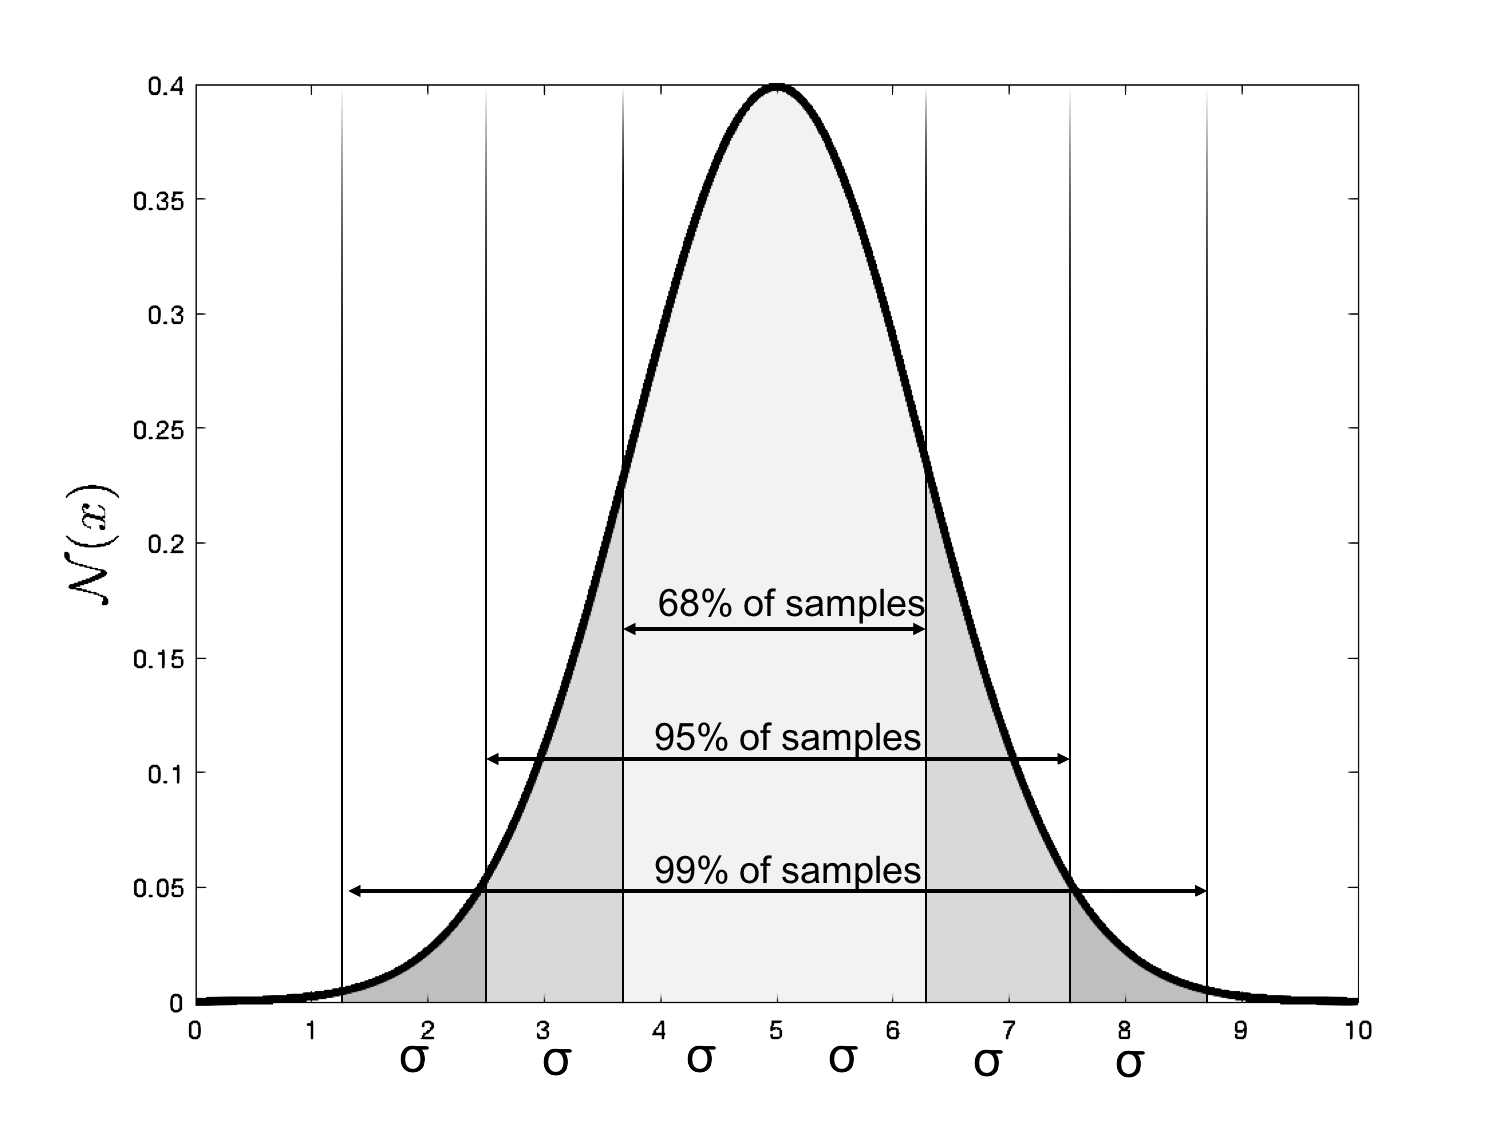
\includegraphics[width=0.4\textwidth]{689599rule.png}
		\vspace{-.5em}
		\caption{68-95-99 rule for Gaussian bell-curve. \alert{$\mathbf{X\sim N(0,\sigma^2)}$}}
	\end{figure}
	\vspace{-.5em}
	
	\begin{columns}
		\begin{column}{.5\textwidth}
			\small
			\textbf{Chebyshev's Inequality:}
			\vspace{-.5em}
			\begin{align*}
				\Pr\left(|X - \E[X]| \geq 1\sigma \right) &\leq 100\% \\
				\Pr\left(|X - \E[X]| \geq 2\sigma \right) &\leq 25\% \\
				\Pr\left(|X - \E[X]| \geq 3\sigma \right) &\leq 11\% \\
				\Pr\left(|X - \E[X]| \geq 4\sigma \right) &\leq 6\%.
			\end{align*}
		\end{column}
		\begin{column}{.5\textwidth}
			\small
			\textbf{Truth:}
			\vspace{-.5em}
			\begin{align*}
				\Pr\left(|X - \E[X]| \geq 1\sigma \right) &\approx 32\% \\
				\Pr\left(|X - \E[X]| \geq 2\sigma \right) &\approx 5\% \\
				\Pr\left(|X - \E[X]| \geq 3\sigma \right) &\approx 1\% \\
				\Pr\left(|X - \E[X]| \geq 4\sigma \right) &\approx .01\%
			\end{align*}
		\end{column}
	\end{columns}
\end{frame}

\begin{frame}
	\frametitle{gaussian concentration}
	\small
	$X \sim \mathcal{N}(\mu,\sigma^2)$ has probability density function (PDF) $p$ with:
	\begin{align*}
		p(\mu \pm x) = \frac{1}{\sigma\sqrt{2\pi}} \alert{\mathbf{e^{-x^2/2\sigma^2}}}
	\end{align*}
	\vspace{-1em}
	\begin{lemma}[Gaussian Tail Bound]
		For $X \sim \mathcal{N}(\mu,\sigma^2)$:\vspace{-.5em}
		\begin{align*}
			\Pr[|X - \E X| \geq k\cdot\sigma] \leq 2e^{-k^2/2}.
		\end{align*}
	\end{lemma}
Compare this to: 
	\begin{lemma}[Chebyshev's Inequality]
	For $X \sim \mathcal{N}(\mu,\sigma^2)$:\vspace{-.5em}
	\begin{align*}
		\Pr[|X - \E X| \geq k\cdot\sigma] \leq \frac{1}{k^2}
	\end{align*}
\end{lemma}
\end{frame}

\begin{frame}
	\frametitle{gaussian concentration}
	\begin{figure}
		\begin{subfigure}[t]{0.47\textwidth}
			\centering
			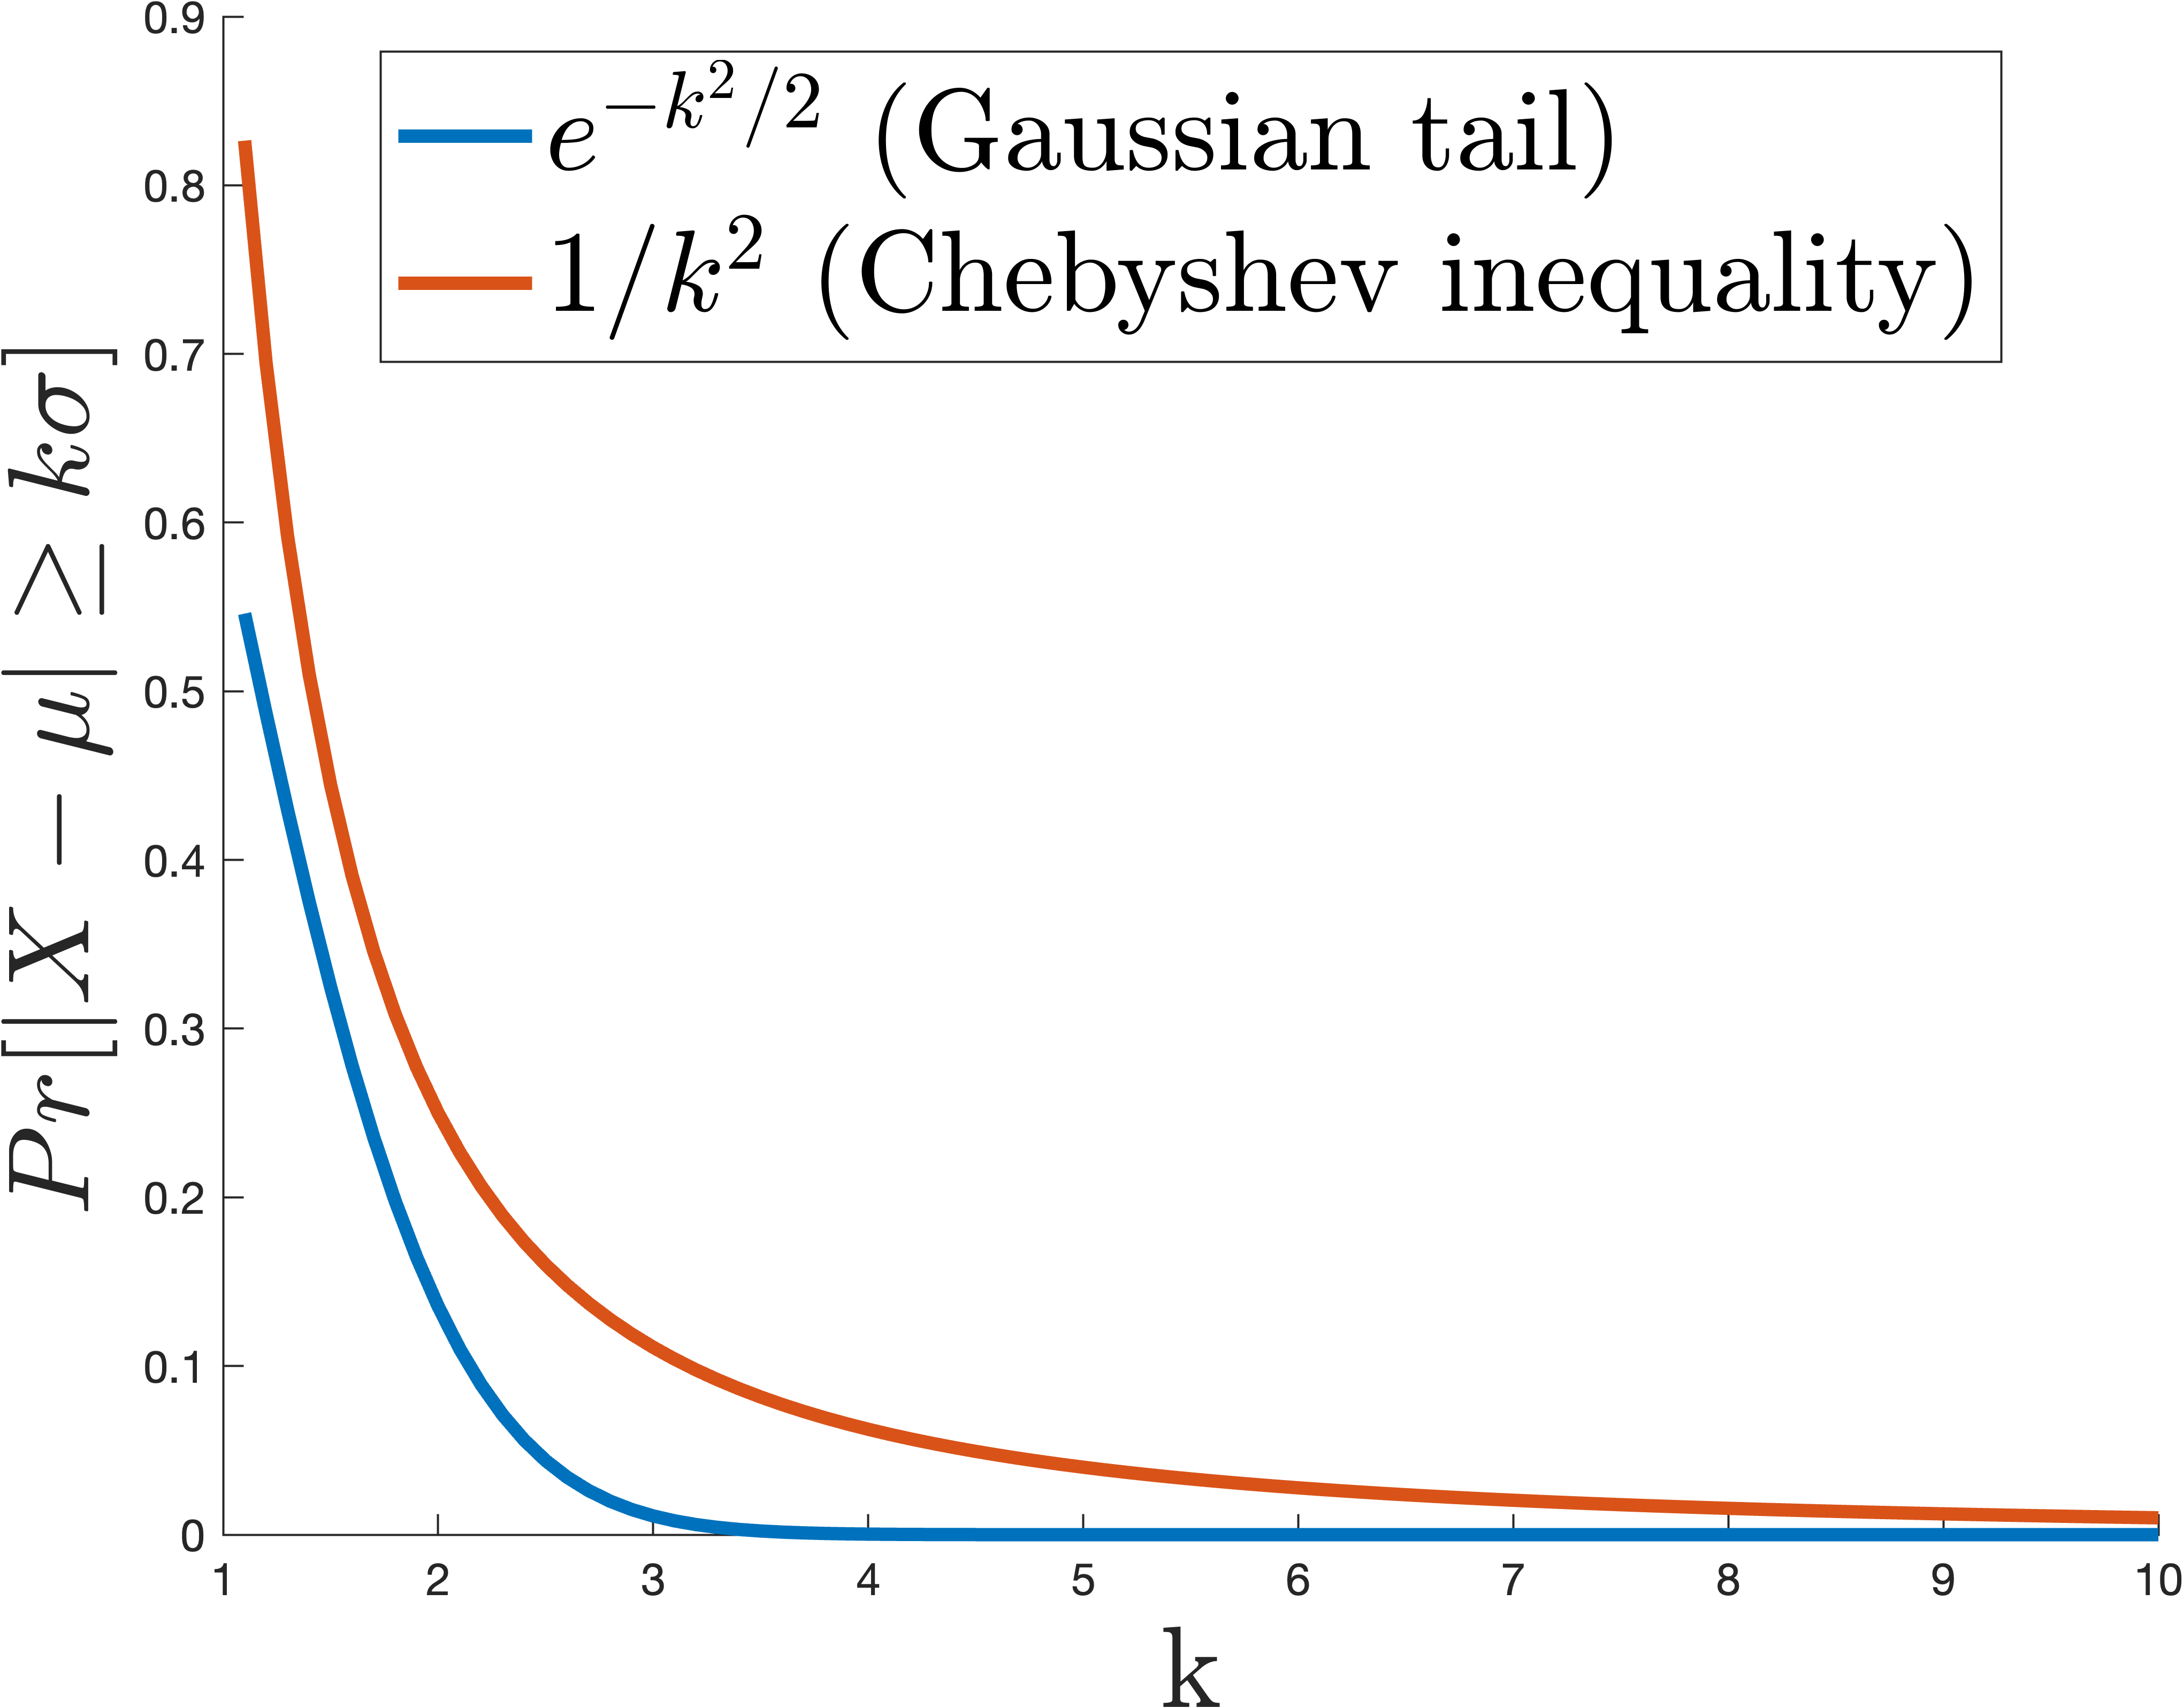
\includegraphics[width=\textwidth]{standardScale.png}
			\caption{Standard $y$-scale.}
		\end{subfigure}
		\hspace{.5em}
		\begin{subfigure}[t]{0.47\textwidth}
			\centering
			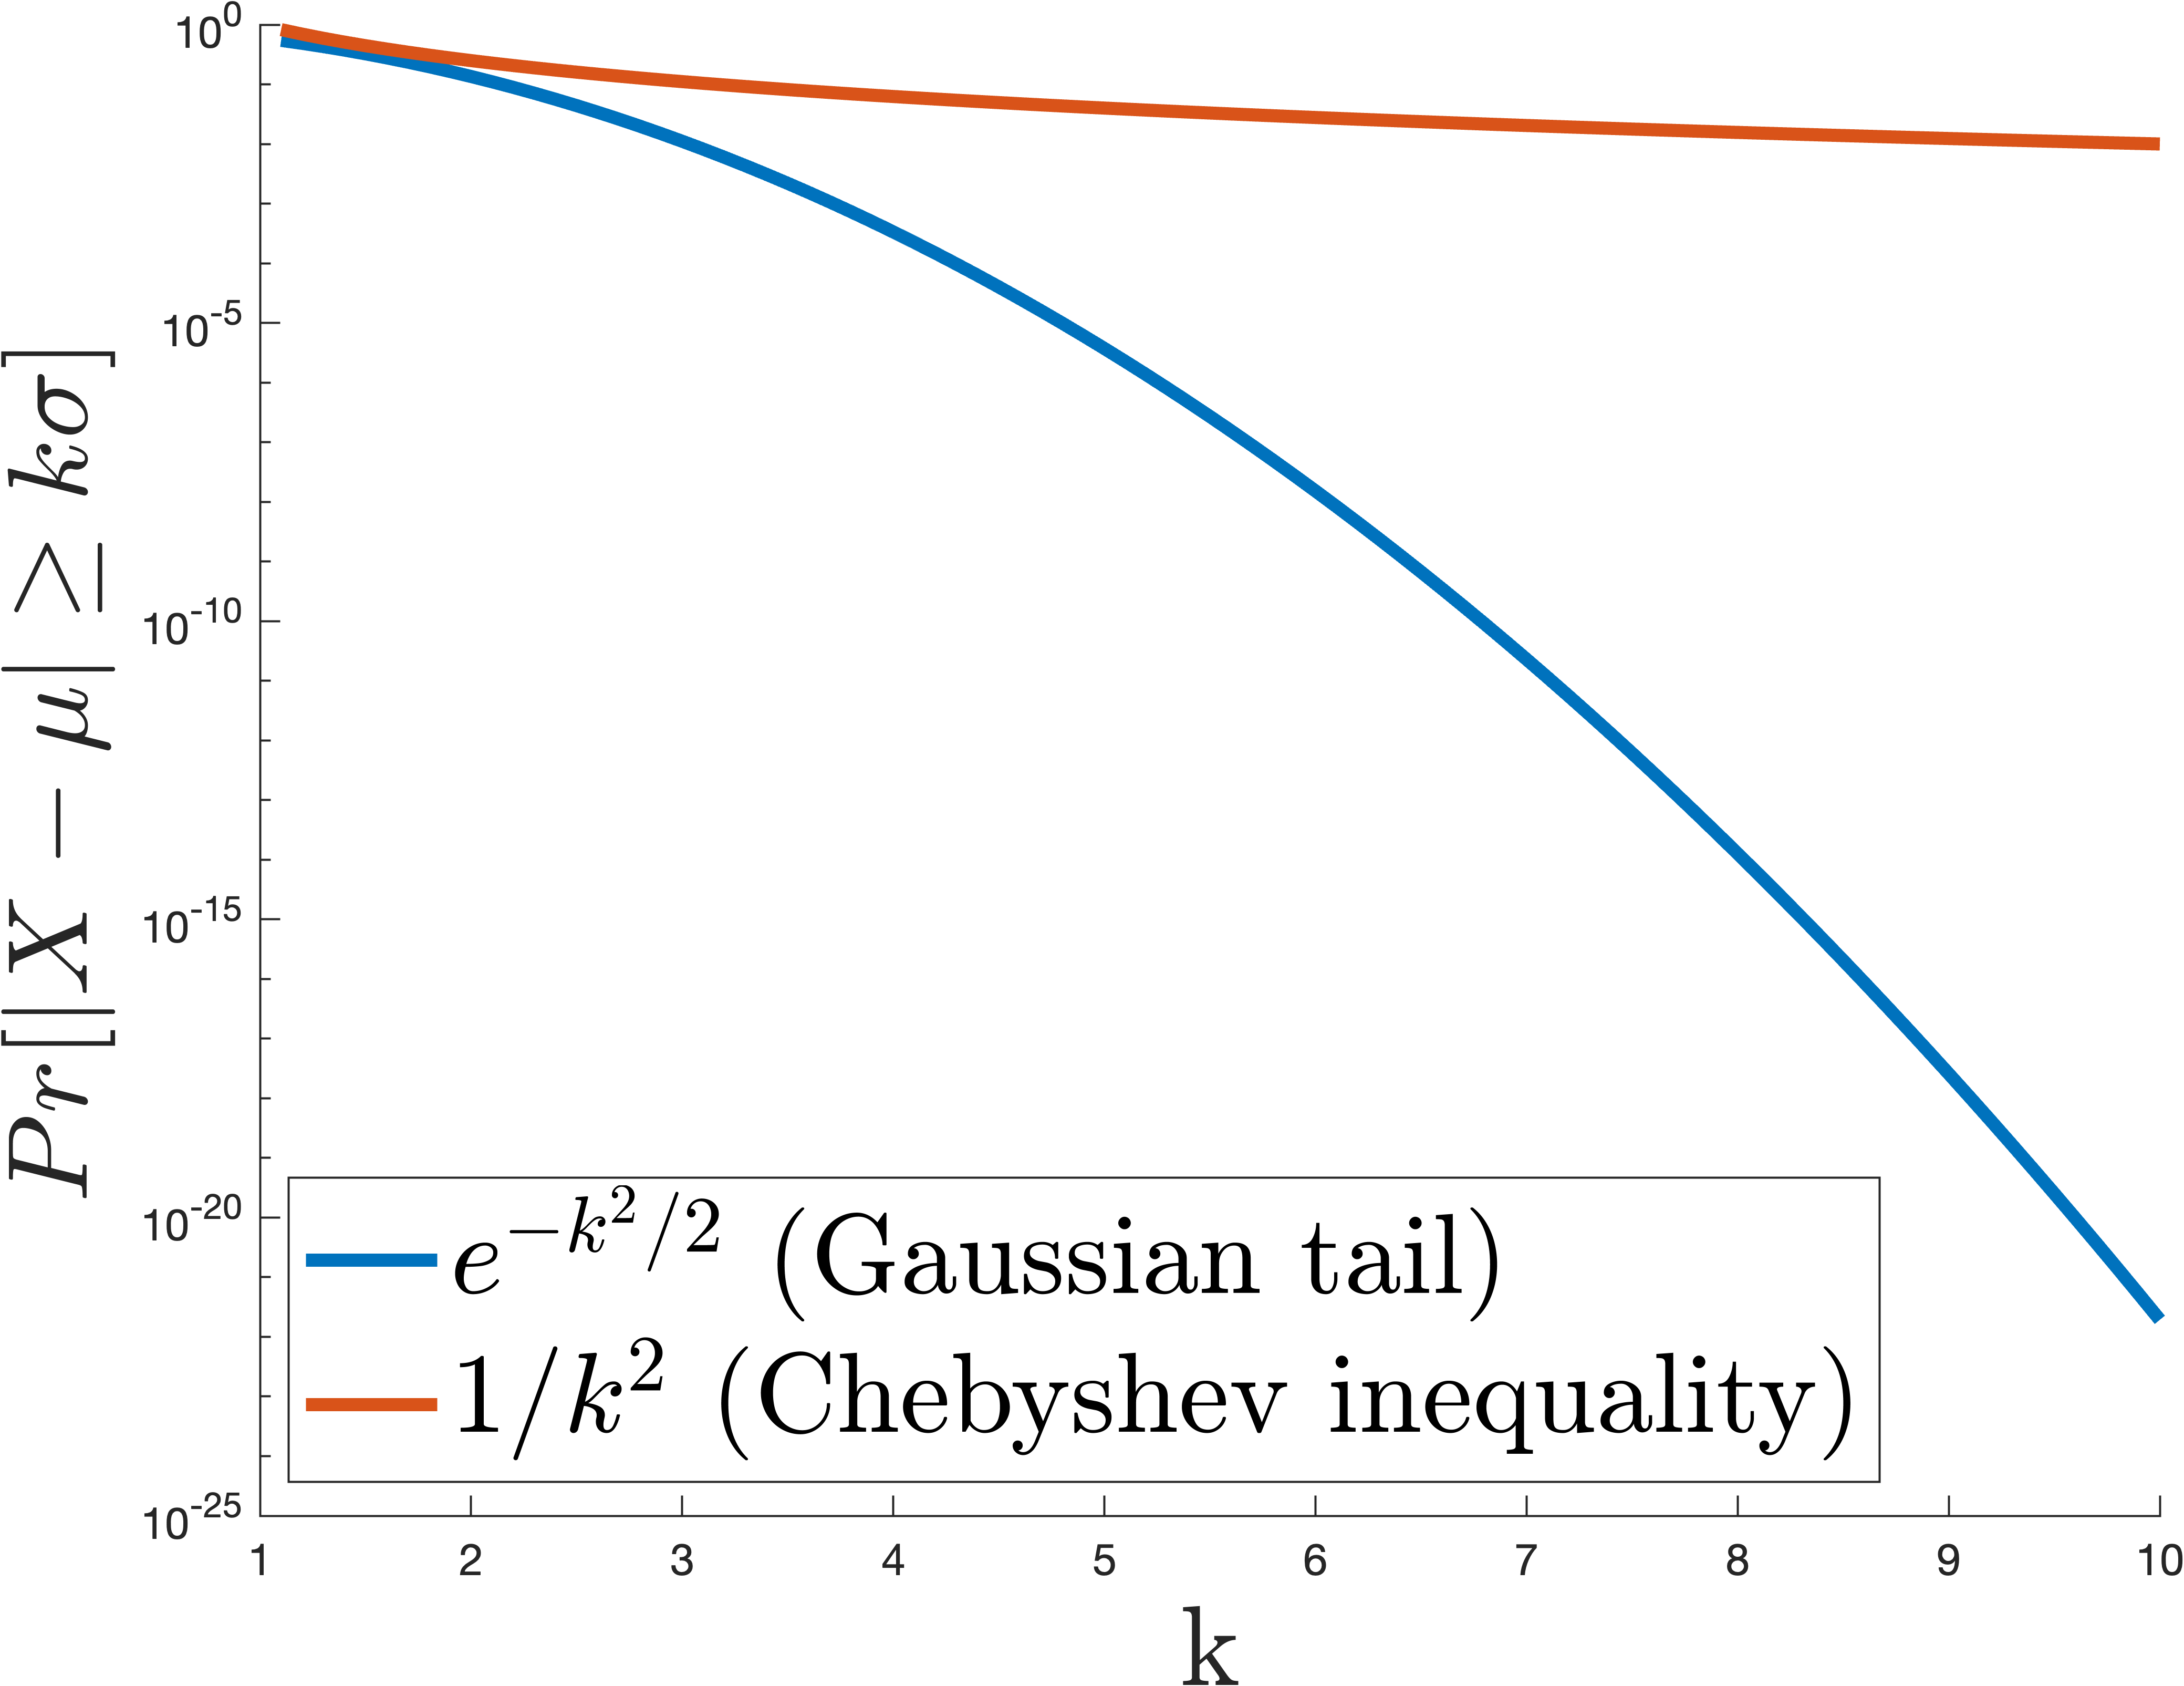
\includegraphics[width=\textwidth]{logScale.png}
			\caption{Logarithmic $y$-scale.}
		\end{subfigure}
	\end{figure}
	\textbf{Takeaway:} Gaussian random variables concentrate much tighter around their expectation than variance alone predicts (i.e., than Chebyshevs's inequality  predicts).

\begin{center}
	\alert{\textbf{Why does this matter for algorithm design?}}
\end{center}
\end{frame}

\begin{frame}
	\frametitle{central limit theorem}
	\begin{theorem}[CLT -- Informal]
		Any sum of \alert{mutually independent}, \alert{(identically distributed)}  r.v.'s $X_1,  \ldots, X_n$ with mean $\mu$ and finite variance $\sigma^2$ converges to a Gaussian r.v. with mean $n\cdot\mu$ and variance $n\cdot\sigma^2$, as $n\rightarrow \infty$.
		\vspace{-.5em}
		\begin{align*}
			S = \sum_{i=1}^n X_i \Longrightarrow \mathcal{N}(n\cdot\mu, n\cdot\sigma^2).
		\end{align*}	
		\vspace{-.5em}	
	\end{theorem}
	\vspace{-.5em}	
	\begin{figure}
		\begin{subfigure}[t]{0.4\textwidth}
			\centering
			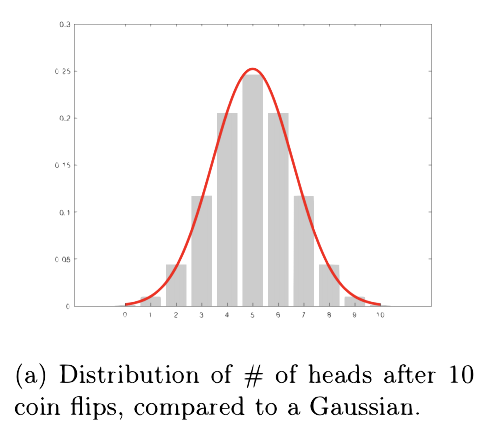
\includegraphics[width=\textwidth]{cltWide.png}
		\end{subfigure}
		\hspace{4em}
		\begin{subfigure}[t]{0.4\textwidth}
			\centering
			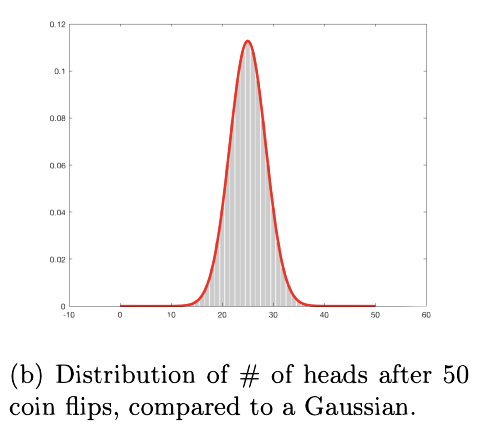
\includegraphics[width=\textwidth]{cltSkinny.png}
		\end{subfigure}
	\end{figure}
\end{frame}

\begin{frame}
	\frametitle{independence}
	Recall:
	\vspace{1em}
	\begin{definition}[Mutual Independence]
		Random variables $X_1, \ldots, X_n$ are \emph{mutually independent} if, for all possible values $v_1, \ldots, v_n$,
		\begin{align*}
			\Pr[X_1 = v_1, \ldots, X_n = v_n] = 	\Pr[X_1 = v_1]\cdot\ldots \cdot\Pr[X_n = v_n]
		\end{align*}
	\end{definition}
	\begin{center}
		\textbf{Strictly stronger than pairwise independence.}
	\end{center}
\end{frame}

\begin{frame}
	\frametitle{exercise}
	\small 
	\begin{center}
		\textbf{If I flip a fair coin $100$ times, lower bound the chance I get between $30$ and $70$ heads?}
	\end{center}
	%	As in the previous lecture, we we would like to use concentration bounds to study the randomized load balancing problem. $n$ jobs are distributed randomly to $n$ servers using a hash function. Let $S_i$ be the number of jobs sent to server $i$. 
	%	\begin{enumerate}[label=(\alph*)]
		%		\item Using the CLT and our lemma for Gaussian concentration, estimate a bound for $\max_i[S_i]$. For example, your bound should take the form: $\Pr[max_i S_i \geq \alert{\textbf{B}}] \leq 1/10$. What's the smallest value of $\textbf{\alert{B}}$ you should hope to achieve? 
		%		\item Last class we proved the above bound with $\textbf{B} = O(\sqrt{n})$ using Chebyshev inequality. How does your bound compare?
		%	\end{enumerate}
	
	Let's approximate the probability by assuming the limit of the CLT holds \emph{exactly} -- i.e., that this sum looks exactly like a Gaussian random variable.
	\begin{lemma}[Gaussian Tail Bound]
		For $X \sim \mathcal{N}(\mu,\sigma^2)$:\vspace{-.5em}
		\begin{align*}
			\Pr[|X - \E X| \geq k\cdot\sigma] \leq 2e^{-k^2/2}.
		\end{align*}
	\end{lemma}
	\vspace{5em}
	$2e^{-8} = .06\%$. Chebyshev's inequality gave a bound of $6.25\%$. 
\end{frame}

%\begin{frame}
%	\frametitle{back-of-the-envelop calculation}
%	
\includegraphics[width=.9\textwidth]{envelope.jpg}
%\end{frame}


\begin{frame}
	\frametitle{quantitative versions of the clt}
	\textbf{These back-of-the-envelop calculations can be made rigorous!}
	\textbf{\alert{Lots of different ``versions'' of bound which do so.}}
		\begin{center}
			\begin{itemize}
				\item Chernoff bound
				\item Bernstein bound
				\item Hoeffding bound
				\item $\ldots$
			\end{itemize}
			Different assumptions on random varibles (e.g. binary vs. bounded), different forms (additive vs. multiplicative error), etc. \textbf{Wikipedia is your friend.}
		\end{center}
\end{frame}

\begin{frame}
	\frametitle{quantitative versions of the clt}
	\begin{theorem}[Chernoff Bound]
		Let $X_1,X_2,\ldots,X_n$ be independent $\{0,1\}$-valued random variables and let
		$p_i = \E[X_i]$, where $0<p_i<1$.
		Then the sum $S = \sum_{i=1}^{n} X_i$, which has mean
		$\mu = \sum_{i=1}^{n} p_i$, satisfies
		\begin{align*}
			\Pr[S \geq (1+\epsilon)\mu] \leq e^{\frac{-\epsilon^2\mu}{2+ \epsilon}}.
		\end{align*}
		and for $0<\epsilon <1$
		\begin{align*}
			\Pr[S \leq (1-\epsilon)\mu] \leq e^{\frac{-\epsilon^2\mu}{2}}.
		\end{align*}
	\end{theorem} 
\end{frame}

\begin{frame}[t]
	\frametitle{chernoff bound}
	\begin{theorem}[Chernoff Bound Corollary]
		Let $X_1,X_2,\ldots,X_n$ be independent $\{0,1\}$-valued random variables and let
		$p_i = \E[X_i]$, where $0<p_i<1$.
		Let $S = \sum_{i=1}^{n} X_i$ and $\E[S] = \mu$. For $\epsilon \in (0,1)$,
		\begin{align*}
				\Pr[|S - \mu| \geq \epsilon \mu] \leq 2e^{-\epsilon^2 \mu/3}
		\end{align*}
	\end{theorem} 
Why does this look like the Gaussian tail bound of 	$\Pr[|S - \mu| \geq k\cdot\sigma] \lesssim 2e^{-k^2/2}$? What is $\sigma(S)$?
\end{frame}



\begin{frame}[t]
	\frametitle{quantitative versions of the clt}
	\begin{theorem}[Bernstein Inequality]
		Let $X_1, X_2, \ldots, X_n$ be independent random variables with each $X_i \in [-1,1]$.
		Let $\mu_i =\E[X_i]$ and $\sigma_i^2 = \Var[X_i]$. Let  $\mu =\sum_{i=1}^n \mu_i$ and $\sigma^2 =\sum_{i=1}^n \sigma_i^2$. Then, for $k \leq \frac{1}{2}\sigma$, $S =\sum_{i=1}^n X_i$ satisfies
		$$\Pr[|S - \mu| > k\cdot \sigma] \leq  2 e^{-{k^2}/{4}}.$$
	\end{theorem}
\end{frame}

\begin{frame}[t]
	\frametitle{quantitative versions of the clt}
	\begin{theorem}[Hoeffding Inequality]
		Let $X_1, X_2, \ldots, X_n$ be independent random variables with each $X_i \in [a_i,b_i]$.
		Let $\mu_i =\E[X_i]$ and $\mu =\sum_{i=1}^n \mu_i$. Then, for any $k > 0$, $S =\sum_{i=1}^n X_i$ satisfies:
		$$\Pr[|S - \mu| > k] \leq  2 e^{\frac{-2k^2}{\sum_{i=1}^n (b_i-a_i)^2}}.$$
	\end{theorem}
\end{frame}

\begin{frame}
	\frametitle{how are these bounds proven?}
	Variance is a natural \emph{measure of central tendency}, but there are others. 
	\begin{align*}
		q^\text{th} \text{ central moment: } \E[(X-\E X)^q]
	\end{align*}
	$q = 2$ gives the variance. Proof of Chebyshev's applies Markov's inequality to the random variable $(X - \E X)^2)$.
	
	\textbf{Idea in brief:} Apply Markov's inequality to $\E[(X-\E X)^q]$ for larger $q$, or more generally to $f(X-\E X)$ for some other non-negative function $f$. E.g., to $\exp(X-\E X)$. Doing so requires higher-order independence.
\end{frame}

\begin{frame}[t]
	\frametitle{exercise}
	\small 
	\begin{center}
		\textbf{If I flip a fair coin $100$ times, lower bound the chance I get between $30$ and $70$ heads?}
	\end{center}
	
		\textbf{Corollary of Chernoff bound}: Let $S = \sum_{i=1}^n X_i$ and $\mu = \E[S]$. For $0< \epsilon < 1$, 
	\vspace{-.75em}
	\begin{align*}
		\Pr[|S - \mu| \geq \epsilon \mu] \leq 2e^{-\epsilon^2 \mu/3}
	\end{align*} 
	Here $X_i = \mathbbm{1}[i^\text{th} \text{ flip is heads}]$. 
	\vspace{8em}
	
	$1.4\%$.
\end{frame}

\begin{frame}[t]
	\frametitle{chernoff bound application}
	\textbf{General Statement:} Flip biased coin $n$ times: i.e. the coin is heads with probability $b$. As long as $n \geq O\left(\frac{\log(1/\delta)}{\epsilon^2}\right)$,
	\vspace{-.5em}
	\begin{align*}
		\Pr[|\text{\# heads} - b\cdot n| \geq \epsilon n] \leq \delta 
	\end{align*}

	

	\vspace{10em}
		Pay very little for higher probability -- if you increase the number of coin flips by 4x, $\delta$ goes from $1/10 \rightarrow 1/100 \rightarrow 1/10000$
\end{frame}

\begin{frame}
	\frametitle{load balancing}
	\textbf{Load balancing problem:}
	
	Suppose Google answers map search queries using servers $A_1, \ldots, A_q$. Given a query like ``new york to rhode island'', common practice is to choose a random hash function $h \rightarrow \{1\ldots, q\}$ and to route this query to server:
	\begin{align*}
		A_{h(\text{``new york to rhode island'})}
	\end{align*}

	\textbf{Goal:} Ensure that requests are distributed evenly, so no one server gets loaded with too many requests. We want to avoid  downtime and slow responses to clients. 
	
	\begin{center}
		\alert{\textbf{Why use a hash function instead of just distributing requests randomly?}}
	\end{center}
	

\end{frame}

\begin{frame}
	\frametitle{load balancing}
	Suppose we have $n$ servers and $m$ requests, $x_1,\ldots, x_m$. Let $s_i$ be the number of requests sent to server $i \in \{1,\ldots, n\}$ :
	\begin{align*}
		s_i = \sum_{j=1}^m \mathbbm{1}[h(x_j) = i]. 
	\end{align*}
	
	Formally, our goal is to understand the value of maximum load on any server, which can be written as the random variable:
	\begin{align*}
		S = \max_{i\in \{1,\ldots, n\}} s_i.
	\end{align*}	
\end{frame}

\begin{frame}
	\frametitle{load balancing}
	A good first step is to first think about expectations. 
	If we have $n$ servers and $m$ requests, for any $i\in \{1,\ldots, n\}$:
	\begin{align*}
		\E[s_i] = \sum_{j=1}^m \E\left[\mathbbm{1}[h(x_j) = i]\right] = \frac{m}{n}.
	\end{align*}
	
	But it's unclear what the expectation of $S = \max_{i\in \{1,\ldots, n\}} s_i$ is... in particular, $\E[S] \alert{\neq} \max_{i\in \{1,\ldots, n\}} \E[s_i]$. 
	
	\textbf{Exercise:} Convince yourself that for two random variables $A$ and $B$, $\E[\max(A,B)] \neq \max(\E[A], \E[B])$ even if those random variable are independent. 
\end{frame}

\begin{frame}
	\frametitle{simplifying assumptions}
	\textbf{Number of servers:} To reduce notation and keep the math simple, let's assume that $m = n$. I.e., we have exactly the same number of servers and requests. 
	
	\textbf{Hash function:} Continue to assume a fully (uniformly) random hash function $h$.
	
	\begin{center}
		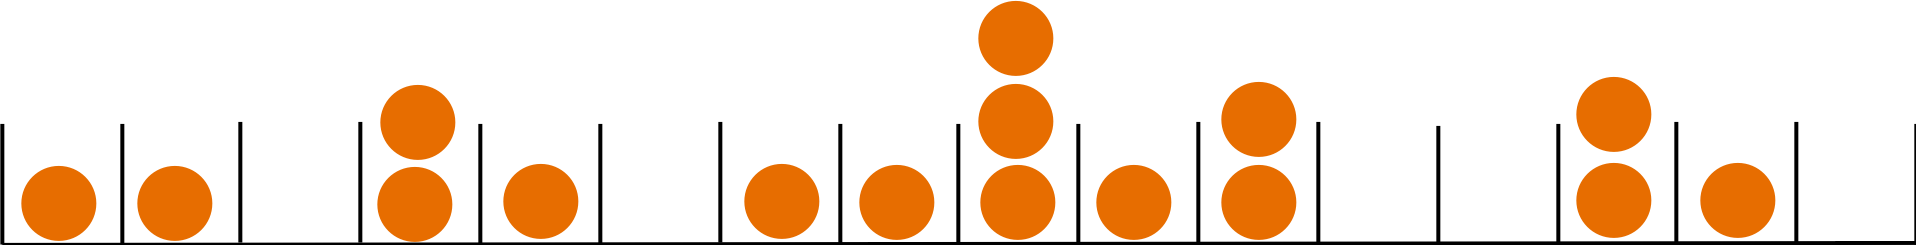
\includegraphics[width=.8\textwidth]{balls_into_bins.png}
		
		Often called the ``balls-into-bins'' model. 
	\end{center}
	
	$\E[s_i] = $ expected number of balls per bin $=\frac{m}{n} = 1$. We would like to prove a bound of the form:
	\begin{align*}
		\Pr[\max_i s_i \geq C] \leq \frac{1}{10}. 
	\end{align*}
	for as tight a value of $C$. I.e., something much better than $C = n$. 
\end{frame}

\begin{frame}
	\frametitle{bounding a union of events}
	\textbf{Goal:} Prove that for some $C$,
	\begin{align*}
		\Pr[\max_i s_i \geq C] \leq \frac{1}{10}. 
	\end{align*}	
	\textbf{Equivalent statement:} Prove that for some $C$, 
	\begin{align*}
		\Pr[(s_1 \geq C) \cup (s_2 \geq C) \cup \ldots \cup (s_n \geq C)] \leq \frac{1}{10}. 
	\end{align*}

	These events are not independent, but we can apply \emph{union bound}!

	\vspace{1em}
	\begin{block}{\vspace*{-3ex}}
		\small $n = $ number of balls and number of bins. $s_i$ is number of balls in bin $i$. $C =$ upper bound on maximum number of balls in any bin.
	\end{block}
\end{frame}

\begin{frame}
	\frametitle{application of union bound}
	We want to prove that:
	\begin{align*}
		\Pr[\max_i s_i \geq C] = \Pr[(s_1 \geq C) \cup (s_2 \geq C) \cup \ldots \cup (s_n \geq C)] \leq \frac{1}{10}. 
	\end{align*}
	
	\alert{To do so, it suffices to prove that for all $i$:
		\begin{align*}
			\Pr[s_i \geq C] \leq \frac{1}{10n}. 
	\end{align*}}
	Why? Because then by the union bound, 
	\begin{align*}
		\Pr[\max_i s_i \geq C] &\leq \sum_{i=1}^n \Pr[s_i \geq C] \text{\hspace{1em}\blue{(Union bound)}}\\
		&\leq \sum_{i=1}^n \frac{1}{10n} = \frac{1}{10}. \qed
	\end{align*}
	

	\begin{block}{\vspace*{-3ex}}
		\small $n = $ number of balls and number of bins. $s_i$ is number of balls in bin $i$.
	\end{block}
\end{frame}

\begin{frame}
	\frametitle{new goal}
	Prove that for some $C$, 
	\begin{align*}
		\Pr[s_i \geq C] \leq \frac{1}{10n}. 
	\end{align*}
	Let's try doing this with Markov's, Chebyshev, and exponential concentration.
\end{frame}


\begin{frame}
	\frametitle{attempt with markov's inequality}
	\vspace{1em}
	\textbf{Goal:} Prove that $\Pr[s_i \geq C] \leq \frac{1}{10n}$. 
	\begin{itemize}
		\item \textbf{Step 1.} Verify we can apply Markov's: $s_i$ takes on non-negative values only. Good to go!
		\item \textbf{Step 2.} Apply Markov's: $\Pr[s_i \geq C] \leq \frac{\E[s_i]}{C} = \frac{1}{C}$. 
	\end{itemize}
	To prove our target statement, need to see $C = 10n$. 
	
	\emph{Meaningless!} There are only $n$ balls, so of course there can't be more than $10n$ in the most overloaded bin. 
	
	\vspace{2em}
	\begin{block}{\vspace*{-3ex}}
		\small $n = $ number of balls and number of bins. $s_i$ is number of balls in bin $i$. $\E[s_i] = 1$. $C =$ upper bound on maximum number of balls in any bin. \textbf{Markov's inequality}: for positive r.v. $X$, $\Pr[X \geq t] \leq \E[X]/t$.  
	\end{block}
\end{frame}

\begin{frame}
	\frametitle{attempt with chebyshev's inequality}
	\textbf{Goal:} Prove that $\Pr[s_i \geq C] \leq \frac{1}{10n}$. 
	\begin{itemize}
		\item \textbf{Step 1.} To apply Chebyshev's inequality, we need to understand $\sigma^2 = \Var[s_i]$. 
	\end{itemize}
	Use \emph{linearity of variance}. Let $s_{i,j}$ be a $\{0,1\}$ indicator random variable for the event that ball $j$ falls in bin $i$. We have:
	\begin{align*}
		s_i = \sum_{j=1}^n s_{i,j}. 
	\end{align*}

	
	\vspace{0em}
	\begin{block}{\vspace*{-3ex}}
		\small $n = $ number of balls and number of bins. $s_i$ is number of balls in bin $i$. $\E[s_i] = 1$. $C =$ upper bound on max number of balls in bin. 
	\end{block}
\end{frame}

\begin{frame}
	\frametitle{variance analysis}

	\begin{align*}
		s_{i,j} = \begin{cases}
			1 \text{ with probability } \frac{1}{n}\\
			0 \text{ otherwise}.
		\end{cases}
	\end{align*}
	\begin{align*}
		\E[s_{i,j}] &= \hspace{10em}\\
		\E[s_{i,j}^2] &=  \hspace{10em}
	\end{align*}
	So:
	\begin{align*}
		\Var[s_i] = \Var\left[\sum_{j=1}^n s_{i,j}\right] = \hspace{15em}
	\end{align*}
	
	\vspace{3em}
	\begin{block}{\vspace*{-3ex}}
		\small $n = $ number of balls and number of bins. $s_{i,j}$ is event ball $j$ lands in bin $i$.
	\end{block}
\end{frame}

\begin{frame}
	\frametitle{applying chebyshev's}
	\textbf{Goal:} Prove that $\Pr[s_i \geq C] \leq \frac{1}{10n}$. 
	
	\textbf{Step 1.} To apply Chebyshev's inequality, we need to understand $\sigma^2 = \Var[s_i]$. 
	\begin{align*}
		\Var[s_i] = \sum_{j=1}^n \Var[s_{i,j}] = \sum_{j=1}^n \frac{1}{n} - \frac{1}{n^2} = {1- \frac{1}{n} \alert{\leq 1}.}
	\end{align*}
	
	\textbf{Step 2.} Apply Chebyshev's inequality:
	\begin{align*}
		&\Pr\left[\left|s_i - \E[s_i]\right| \geq k\cdot 1\right] \leq \frac{1}{k^2}
	\end{align*}
	
	\vspace{0em}
	\begin{block}{\vspace*{-3ex}}
		\small $n = $ number of balls and number of bins. $s_i=$ number of balls in bin $i$.  $s_{i,j}$ is event ball $j$ lands in bin $i$. $\E[s_i] = 1$. 
	\end{block}
\end{frame}

\begin{frame}
	\frametitle{applying chebyshev's}
	\textbf{Goal:} Prove that $\Pr[s_i \geq C] \leq \frac{1}{10n}$. 
	
	We just proved that, for any $k$: \blue{$\Pr[\left|s_i - 1\right| \geq k] \leq \frac{1}{k^2}$.}
	\vspace{12em}
	% Setting $k = \sqrt{10n}$ gives: 
	% \begin{align*}
	% 	\Pr[\left|s_i - 1\right| &\geq \sqrt{10n}] \leq \frac{1}{10 n}.
	% \end{align*}
	% So, we have that:
	% \begin{align*}
	% 	\alert{\Pr[s_i \geq \sqrt{10n} + 1] \leq \frac{1}{10n}.}
	% \end{align*}
	% By the union bound argument from earlier, it thus holds that:
	% \begin{align*}
	% 	\Pr[\max_{i\in \{1,\ldots, n\}}s_i \geq \sqrt{10n} + 1] \leq \frac{1}{10}.
	% \end{align*}
	
	
	\vspace{1em}
	\begin{block}{\vspace*{-3ex}}
		\small $n = $ number of balls and number of bins. $s_i$ is number of balls in bin $i$. $C =$ upper bound on maximum number of balls in any bin.
	\end{block}
\end{frame}

\begin{frame}
	\frametitle{final result for chebyshev's}
	
	\begin{center}
		When hashing $n$ balls into $n$ bins, the maximum bin contains $o(\sqrt{n})$ balls with probability $\frac{9}{10}$.
		
		\vspace{1em}
		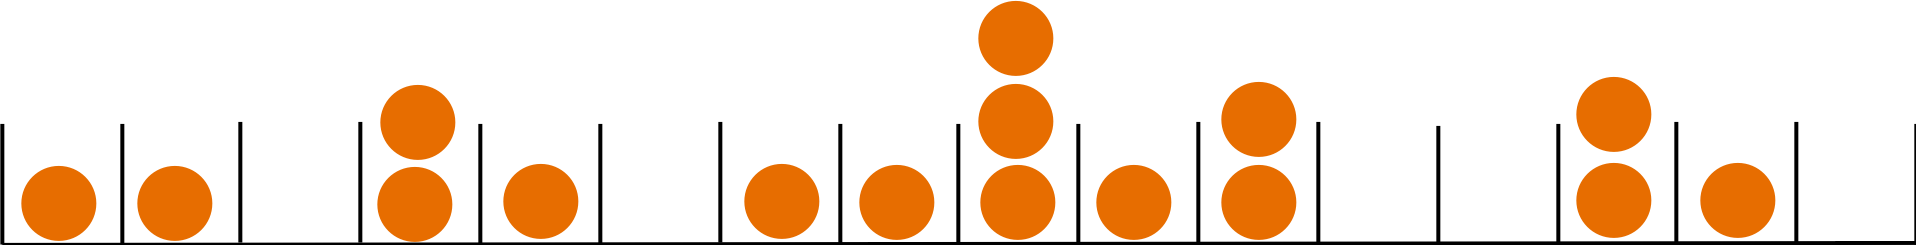
\includegraphics[width=.8\textwidth]{balls_into_bins.png}
		\vspace{1em}
		
		Much better than the trivial bound of $n$! 
	\end{center}
\end{frame}

\begin{frame}[t]
	\frametitle{attempt with exponential concentration}
	\textbf{Goal:} Prove that $\Pr[s_i \geq C] \leq \frac{1}{10n}$. 
	
	\textbf{Recall:} $s_i = \sum_{j=1}^n s_{i,j}$, where $s_{i,j} = \mathbbm{1}[\text{ball $j$ lands in bin $i$}]$.

	\begin{center}
	What bound might we use?
	\end{center}

\end{frame}

\begin{frame}[t]
	\frametitle{attempt with exponential concentration}
	\begin{theorem}[Chernoff Bound]
		Let $X_1,X_2,\ldots,X_n$ be independent $\{0,1\}$-valued random variables and let
		$p_i = \E[X_i]$, where $0<p_i<1$.
		Then the sum $S = \sum_{j=1}^{n} X_i$, which has mean
		$\mu = \sum_{j=1}^{n} p_i$, satisfies
		\begin{align*}
			\Pr[S \geq (1+\epsilon)\mu] \leq e^{\frac{-\epsilon^2\mu}{2+ \epsilon}}.
		\end{align*}
	\end{theorem} 
	Apply with $S = s_i$, $X_j = s_{i,j}$.
	\begin{align*}
		\Pr[S \geq (1+c\log n)\mu] \leq \hspace{18em}
	\end{align*}
	
\end{frame}

\begin{frame}
	\frametitle{load balancing}
	\begin{center}\alert{\textbf{So max load for randomized load balancing is $O(\log n)$!}} Best we could prove with Chebyshev's was $O(\sqrt{n})$. \end{center}
\end{frame}

\begin{frame}
	\frametitle{power of two choices}
	\textbf{Power of 2 Choices:} Instead of assigning job to random server, choose 2 random servers and assign to the least loaded. With probability $1/10$ the maximum load is bounded by:
	
	(a) $O(\log n)$ \hspace{1em} (b) $O(\sqrt{\log n})$  \hspace{1em}  (c) $O(\log \log n)$  \hspace{1em} (d) $O(1)$
	\begin{center}
		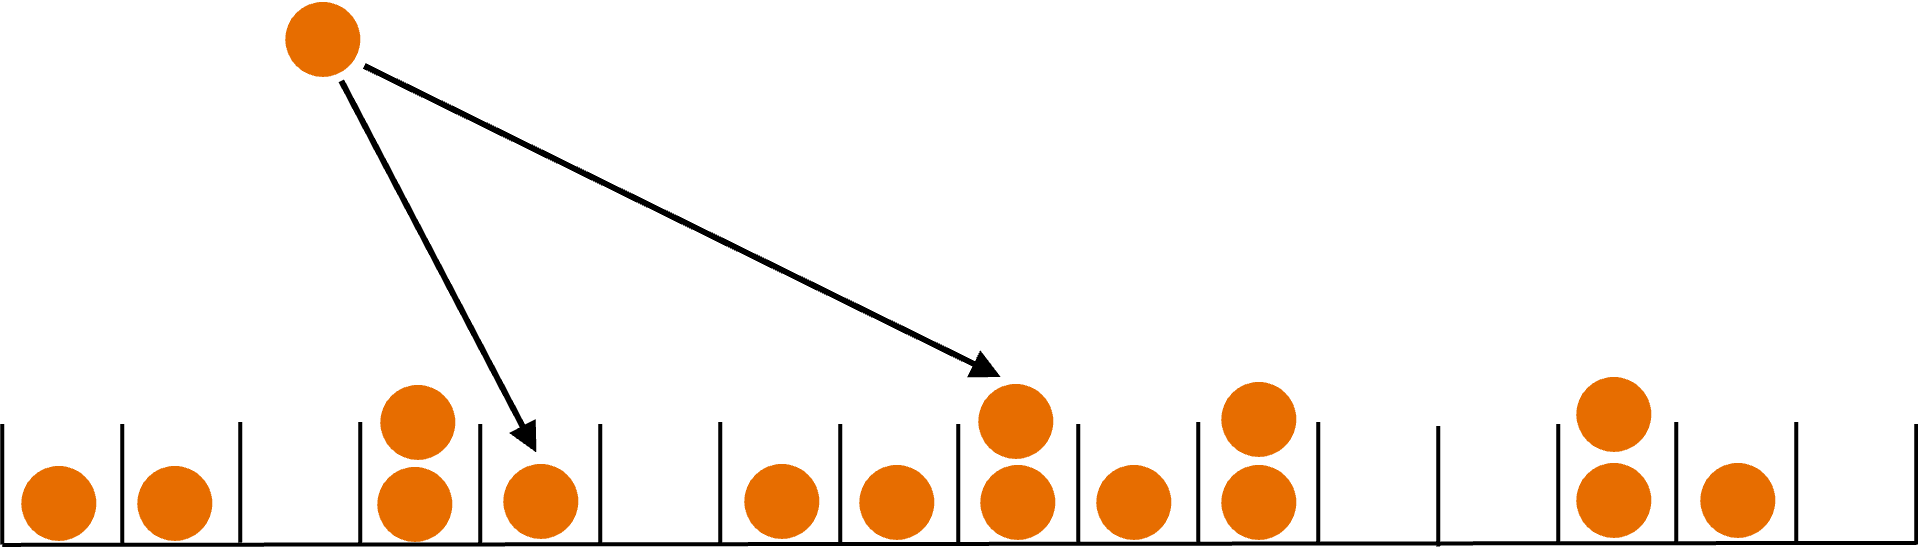
\includegraphics[width=.9\textwidth]{power_of_two.png}
	\end{center}
\end{frame}



\end{document} 




